\subsection{Problem: Extracting Code Template from \stackoverflow.} 
In order to extract the templates from the \stackoverflow we need to:
\begin{enumerate}
	\item Identify the code with potential of reusability inside the code snippet and 
    \item Structure the code into a reusable form (template).  
\end{enumerate}

\subsection{Extracting Code.}
In terms of a SO question, we define the code with potential reusability as the \textit{solution} for the inquired question.
\begin{itemize}
	\item Identifying the solution of a \stackoverflow question is by itself a very hard problem.
    \item Context dependent. To completely solve this issue we would be required to understand the usage context of the code.
    \item We restrict the domain of the problem by focusing only on API-related questions.
\end{itemize}

% Pandas Study Case



\textbf{Pandas Study Case.}
% In this section we will describe the study case of the top 100 Pandas related questions in \stackoverflow.  
We perform a case study by manually analyzing the top 100 most viewed questions in \stackoverflow related to Pandas API.
Pandas is an open source library for data analysis in Python~\footnote{https://pandas.pydata.org/}.

\textbf{Why most viewed questions?}
We do not claim that the most viewed questions are representative of the average \stackoverflow question/answer.
The most viewed questions provide solutions to problems more frequently asked by developers, and templates generated from those questions have a higher chance of being used in a real development scenario.
Also, we expect that 

There are two components in this problem:
\begin{itemize}
	\item Code Snippet: the entire code embedded in a \stackoverflow response.
    \item Solution: the reusable code that needs to be identified. \diego{this will be better defined}
\end{itemize}

To better understand the problem of extracting the solution from a code snippet, we characterize the relation between code snippet and solution into four cases:

%complexity of extracting the solution through the relation of the code snippet and the solution properties.
% We found four distinct cases

\textbf{Case 1. Single-line snippet.}  
Trivial case, where the snippet is comprised by a single statement. 
In this particular case, the entire code snippet is the solution (see \ref{lst:case1}).


\textbf{Case 2. Multi-line snippet and single-line solution.}
Case where the code snippet contain unessential code that needs to be filtered for a template. 
The extra code is often related to the setup of the scenario and I/O operations for printing the outcome of the solution code. 

\textbf{Case 3. Multi-line snippet and Multi-line solution.}
Similar to case 2, but the solution is spread in multiple lines of code.
% The challenge of creating templates for this case of snippet and solution, is that the app

\textbf{Case 4. Multi-line snippet and Multiple Alternative solutions.}
Some \stackoverflow answers provide multiple solutions to the question.
This case is particularly challenging as the semantic of the solution needs to be inferred in order to identify multiple alternative solutions.
For instance, the case depicted in~\Cref{fig:daatset-cases} showcase the complex task of extracting both alternative solutions.

% The Most viewed pandas related question in SO provides two distinctive ways for renaming pandas columns.
% The only difference of those two API calls is the \texttt{inplace}.


% \begin{enumerate}
% 	\item Single-line snippet. 
%     \item Multi-line snippet - Single-line solution.
%     \item Multi-line snippet - Multi-line solution.
%     \item Multi-line snippet - Alternative solutions.
	
% \end{enumerate}

\begin{figure*}[tbh]
\label{fig:daatset-cases}
\caption{Examples of \stackoverflow code }
\begin{subfigure}{0.5\textwidth}
\begin{lstlisting}[title={Case 1. Single line code snippet.}, label={lst:case1}, captionpos = b]
# Question: Filter dataframe rows if value in column is in a set list of values
rpt[rpt['STK_ID'].isin(stk_list)]
\end{lstlisting}
\end{subfigure}
~
\begin{subfigure}{0.5\textwidth}
\begin{lstlisting}[title={Case 2. Single line solution code.}, label={lst:case2}, captionpos = b]
# Question: Use a list of values to select rows from a pandas dataframe [duplicate]
# Setup
In [5]: df = DataFrame({'A' : [5,6,3,4], 'B' : [1,2,3, 5]})
# Solution
In [7]: df[df['A'].isin([3, 6])]
\end{lstlisting}
\end{subfigure}  

\begin{subfigure}{0.5\textwidth}
\begin{lstlisting}[title={Case 3. Multi-line solution code}, label={lst:case3}, captionpos = b]
# Question: Import multiple csv files into pandas and concatenate into one DataFrame 
# Setup
path =r'C:\DRO\DCL_rawdata_files' 
allFiles = glob.glob(path + "/*.csv")
# Solution
frame = pd.DataFrame()
list_ = []
for file_ in allFiles:
    df = pd.read_csv(file_,index_col=None, header=0)
    list_.append(df)
frame = pd.concat(list_)
\end{lstlisting}
\end{subfigure}
~
\begin{subfigure}{0.5\textwidth}
\begin{lstlisting}[title={Case 4. Multiple solutions in the snippet (13413590)}, label={lst:case4}, captionpos = b]
# Question: How to drop rows of Pandas DataFrame whose value in certain columns is NaN 

# Alternative 1
df = df[np.isfinite(df['EPS'])]
# Alternative 2
df = df.dropna()
\end{lstlisting}
\end{subfigure}

\end{figure*}


\begin{table}[b]
\label{tab:pandas-top100-analysis}
\caption{Top 100 most viewed Pandas question dataset.}
\begin{tabular}{l l l l}
		 \textbf{Analyzed} 		& \textbf{Objective} 		& \textbf{Answers} 	& \textbf{Total}		\\ 
         \textbf{Questions}		& \textbf{Questions}		&					& \textbf{Solutions}	\\ \hline
		 	100						& 90					& 95				& 219					\\ 
% Category 1	 &							
% Dataset      & 	--						& --						& 52			\\ 

\end{tabular}
\end{table}

\begin{figure}[tbh]
\label{fig:pandas-top100-analysis}
\caption{}
\centering
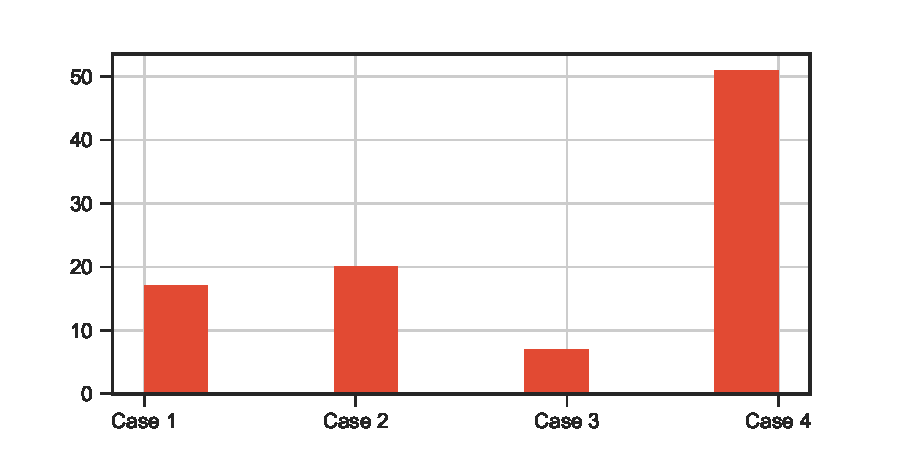
\includegraphics[width=0.45\textwidth]{figures/dataset_cases}
\caption{Preliminary results of current methods evaluated on Statement Granularity.}
\label{fig:dataset-cases}
\end{figure}


% It is important to mention, however, the most viewed questions are not representative of the entire \stackoverflow forum, but provide high quality answers and are (intuitively) the most suitable answers to 

\textbf{Methodology.} We manually analyze the answers to the most viewed Pandas question in \stackoverflow in the following manner:
\begin{enumerate}
	\item We only consider objective questions that have a source-code as the answer. Questions such as \diego{"Add here an example"} were not considered in this analysis. From the initial set, 10 questions were filtered out. 
	\item For each question, we analyze the \textit{accepted answer} and the \textit{most voted answer}, as in some cases, the accepted answer is not the most voted by the community. 5 questions have different most voted/accepted answers, hence we have a total of 95 answers to analyze.
    \item We extract the code snippet and filter out any non-parseable Python code. This step is done to remove comments, special characters from terminal code eg. \texttt{In} and \texttt{Out}, and any code output.
    \item We extract the solution by marking the lines we as developers would copy to use the solution in our own code. \diego{We need a crisp definition here...}
    \item We then classify each answer into one of the four categories presented.
\end{enumerate}

\textbf{Results. }
We present the analysis of the top 100 most viewed in \Cref{fig:pandas-top100-analysis}. 
\begin{itemize}
	\item Multiple Alternative Solutions (case 4) is the most prominent case with $\approx{54\%}$ of the answers. The most viewed questions often have well described answers with multiple alternatives. This shows the importance of an approach that can identify such cases.
    \item Single-line solution in Multi-line snippet was the second most common case with $\approx{21\%}$ of the analyzed answers.
    \item Trivial cases (Single-line snippet) appeared in third with $\approx{17\%}$ of the answers
    \item Multi-line appear only on $\approx{8\%}$ of the answers. 
\end{itemize}


% \begin{lstlisting}[caption={Setup embedded in the solution code (10715965).}, captionpos = b]
% # Question: Filter dataframe rows if value in column is in a set list of values

% df = pd.DataFrame(columns=['lib', 'qty1', 'qty2'])
% for i in range(5):
% 	df.loc[i] = [randint(-1,1) for n in range(3)]
% \end{lstlisting}

% \begin{lstlisting}[caption={Multiple alternatives solution in the snippet (11346283).}, captionpos = b]
% # Question: Renaming columns in pandas

% # Alternative 1
% df = df.rename(columns={'oldName1': 'newName1', 'oldName2': 'newName2'})
% # Alternative 2 
% df.rename(columns={'oldName1': 'newName1', 'oldName2': 'newName2'}, inplace=True)
% \end{lstlisting}








\subsection{Structuring Code}
Given that we have identified the solution code of a \stackoverflow question, we need to normalize the code and structure in a form that can be further reused semi-automatically \diego{maybe automatically?}.

\begin{itemize}
	\item Context dependent. Similarly to the Extracting Code problem to be able to normalize 
    \item Approach the problem in a API-centric way
    \begin{itemize}	
    	\item Identify the API calls as an entry-point.
        \item Use the API documentation to extract and normalize variable names.
    \end{itemize}
\end{itemize}







